\documentclass[landscape,a4paper]{article}

\usepackage{enumerate}
\usepackage{amsmath}
\usepackage{amssymb}
\usepackage{array}
\usepackage{arydshln}
\usepackage{multirow}
\usepackage{multicol}
\usepackage{geometry}
\usepackage{graphicx}

\geometry{left=1cm,right=1cm,top=1cm,bottom=1cm}


\begin{document}

\begin{multicols}{3}
\footnotesize

\section*{Common}
$${\rm sinc\,}\theta=\frac{\sin\pi\theta}{\pi\theta}$$
$$\int e^{at}dt=\frac{1}{a}e^{at}+C$$
$$\int te^{at}dt=\frac{at-1}{t^2}e^{at}+C$$
$$\int t^ne^{at}dt=\frac{t^n}{a}e^{at}-\frac{n}{a}\int t^{n-1}e^{at}dt$$
$$\int e^{at}\sin btdt=\frac{1}{a^2+b^2}e^{at}(a\sin bt-b\cos bt)+C$$
$$\int e^{at}\cos btdt=\frac{1}{a^2+b^2}e^{at}(b\sin bt+a\cos bt)+C$$


\section*{Chapter 3}
\subsection*{Continuous}
$$x(t)=\sum_{k=-\infty}^{+\infty}a_ke^{jk\omega_0t}=\sum_{k=-\infty}^{+\infty}a_ke^{jk(2\pi/T))t}$$
$$a_k=\frac{1}{T}\int_Tx(t)e^{-j\omega_0t}dt=\frac{1}{T}\int_Tx(t)e^{-j(2\pi/T)t}dt$$
$$a_0=\frac{1}{T}\int_Tx(t)dt$$

\subsection*{Convergent}
$$\int_T|x(t)|dt<\infty$$

\subsection*{Discrete}
$$x[n]=\sum_{k=<N>}a_ke^{jk\omega_0n}=\sum_{k=<N>}a_ke^{jk(2\pi/N)n}$$
$$a_k=\frac{1}{N}\sum_{k=<N>}x[n]e^{-jk\omega_0n}=\frac{1}{N}\sum_{k=<N>}x[n]e^{-jk(2\pi/N)n}$$

\section*{Chapter 4}

\subsection*{Continuous}
$$x(t)=\frac{1}{2\pi}\int_{-\infty}^{+\infty}X(j\omega)e^{j\omega t}d\omega$$
$$X(j\omega)=\int_{-\infty}^{+\infty}x(t)e^{-j\omega t}dt$$

\subsection*{Periodic}
$$x(t)=\sum_{k=-\infty}^{+\infty}a_ke^{jk\omega_0t}$$
$$X(j\omega)=\sum_{k=-\infty}^{+\infty}2\pi a_k\delta(\omega-k\omega_0)$$

\subsection*{Differential Equations}

$$\frac{d^2y(t)}{dt^2}+4\frac{dy(t)}{dt}+3y(t)=\frac{dx(t)}{dt}+2x(t)$$
$$H(j\omega)=\frac{(j\omega)+2}{(j\omega)^2+4(j\omega)+3}=\frac{1/2}{j\omega+1}+\frac{1/2}{j\omega+3}$$
$$h(t)=\frac{1}{2}e^{-t}u(t)+\frac{1}{2}e^{-3t}u(t)$$

\section*{Chapter 5}

\subsection*{Discrete}
$$x[n]=\frac{1}{2\pi}\int_{2\pi}X(e^{j\omega}e^{j\omega n})d\omega$$
$$X(e^{j\omega})=\sum_{n=-\infty}^{\infty}x[n]e^{-j\omega n}$$

\subsection*{Periodic}
$$x[n]=\sum_{k=<N>}a_ke^{jk(2\pi/N)n}$$
$$X(e^{j\omega})=\sum_{k=-\infty}^{\infty}2\pi a_k\delta\left(\omega-\frac{2\pi k}{N}\right)$$

\subsection*{Differential Equations}
$$y[n]-\frac{3}{4}y[n-1]+\frac{1}{8}y[n-2]=2x[n]$$
$$H(e^{j\omega})=\frac{2}{1-\frac{3}{4}e^{-j\omega}+\frac{1}{8}e^{-j2\omega}}=\frac{4}{1-\frac{1}{2}e^{-j\omega}}-\frac{2}{1-\frac{1}{4}e^{-j\omega}}
$$
$$h[n]=4\left(\frac{1}{2}\right)^nu[n]-2\left(\frac{1}{4}\right)^nu[n]$$

\section*{Chapter 6}

\subsection*{Group Delay}
$$\tau(\omega)=-\frac{d}{d\omega}\{\sphericalangle H_2{j\omega}\}$$

\subsection*{Step response}
$$s(t)=\int_{-\infty}^th(\tau)d\tau$$
$$s[n]=\sum_{m=-\infty}^{n}h[m]$$

\subsection*{First Order Systems}
$$\tau\frac{dy(t)}{dt}+y(t)=x(t)$$
$$H(j\omega)=\frac{1}{j\omega\tau+1}$$
$$h(t)=\frac{1}{\tau}e^{-t/\tau}u(t)$$
$$s(t)=h(t)*u(t)=[1-e^{-t/\tau}]u(t)$$

\subsection*{Second Order Systems}
$$\frac{d^2y(t)}{dt^2}+2\xi\omega_n^2\frac{dy(t)}{dt}+\omega_n^2y(t)=\omega_n^2x(t)$$
For $\xi\neq1$,
$$H(j\omega)==\frac{M}{j\omega-c_1}-\frac{M}{j\omega-c_2}$$
$$c_{1,2}=-\xi\omega_n\pm\omega_n\sqrt{\xi^2-1},M=\frac{\omega_n}{2\sqrt{\xi^2-1}}$$
$$h(t)=M[e^{c_1t}-e^{c_2t}]u(t)$$
$$s(t)=h(t)*u(t)=\left\{1+M\left[\frac{e^{c_1t}}{c_1}-\frac{e^{c_2t}}{c_2}\right]\right\}u(t)$$
For $\xi=1$,
$$H(j\omega)=\frac{\omega_n^2}{(j\omega+\omega_n)^2}$$
$$h(t)=\omega_n^2te^{-\omega_nt}u(t)$$
$$s(t)=[1-e^{-\omega_nt}-\omega_nte^{-\omega_nt}]u(t)$$
For $0<\xi<1$,
$$H(j\omega)=\frac{1}{(j\omega/\omega_n)^2+2\xi(j\omega/\omega_n)+1}$$
$$h(t)=\frac{\omega_ne^{-\xi\omega_nt}}{\sqrt{1-\xi^2}}[\sin(\omega_n\sqrt{1-\xi^2})t]u(t)$$

\begin{center}
\begin{tabular}{rl}
	$0<\xi<1$ & under damped \\
	$\xi=1$ & critical damped \\
	$\xi>1$ & over damped \\
\end{tabular}
\end{center}

$$\omega_{max}=\omega_n\sqrt{1-2\xi^2}$$
$$|H(j\omega_{max})=\frac{1}{2\xi\sqrt{1-\xi^2}}$$

\end{multicols}


\setcounter{section}{6}

\pagestyle{empty}

\begin{multicols}{3}
\footnotesize

\section{Sampling}

\subsection{The Sampling Theorem}

\subsubsection{Impulse-Train Sampling}
$$x_p(t)=x(t)p(t)$$
$$p(t)=\sum_{n=-\infty}^{+\infty}\delta(t-nT)$$
$$x_p(t)=\sum_{n=-\infty}^{+\infty}x(nT)\delta(t-nT)$$
$$X_p(j\omega)=\frac{1}{2\pi}\int_{-\infty}^{+\infty}X(j\theta)P(j(\omega-\theta))d\theta$$
$$P(j\omega)=\frac{2\pi}{T}\sum_{k=-\infty}^{+\infty}\delta(\omega-k\omega_s)$$
$$X_p(j\omega)=\frac{1}{T}\sum_{k=-\infty}^{+\infty}X(j(\omega-k\omega_s))$$

Sampling Theorem:

Let $x(t)$ be a band-limited signal with $X(j\omega)=0$ for $|\omega|>\omega_M$. Then $x(t)$ is uniquely determined by its samples $x(nT)$, $n=0,\pm1,\pm2,\dots$, if $$\omega_s>2\omega_M$$ where $$\omega_s=\frac{2\pi}{T}$$

Then we can reconstruct $x(t)$ with an ideal lowpass filter with gain $T$ and cutoff frequency $\omega_M<\omega_c<\omega_s-\omega_M$.

\subsubsection{Sampling with a Zero-Order Hold}
$$H_0(j\omega)=e^{-j\omega T/2}\left[\frac{2\sin(\omega T/2)}{\omega}\right]$$
$$H_r(j\omega)=\frac{e^{j\omega T/2}H(j\omega)}{\frac{2\sin(\omega T/2)}{\omega}}$$

\subsection{Interpolation}
$$x_r(t)=x_p(t)*h(t)=\sum_{n=-\infty}^{+\infty}x(nT)h(t-nT)$$
$$h(t)=\frac{\omega_cT\sin(\omega_c t)}{\pi\omega_ct}$$
$$x_r(t)=\sum_{n=-\infty}^{+\infty}x(nT)h\frac{\omega_cT\sin(\omega_c(t-nT))}{\pi\omega_c(t-nT)}$$
$$H(j\omega)=\frac{1}{T}\left[\frac{\sin(\omega T/2)}{\omega/2}\right]^2$$

\subsection{Aliasing}
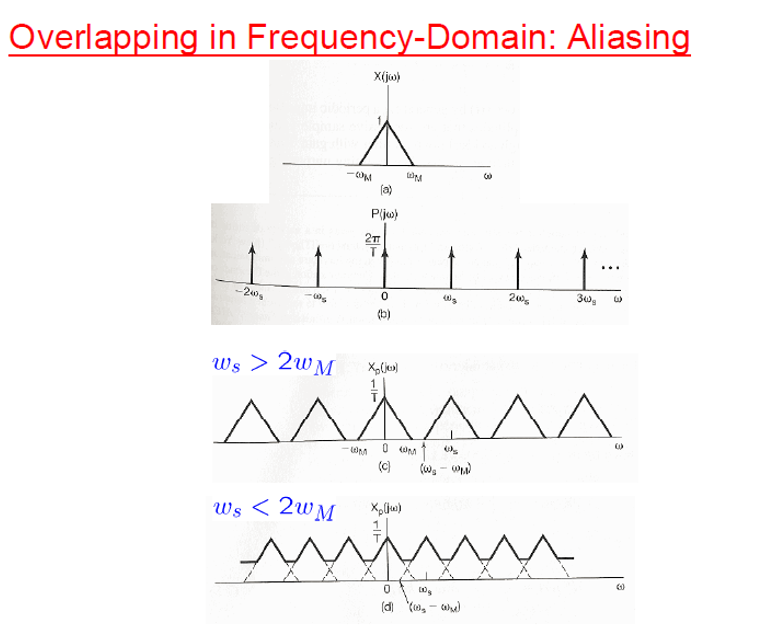
\includegraphics[width=\linewidth]{7.3.png}

\section{Communication Systems}

\subsection{Amplitude Modulation}
$$y(t)=x(t)c(t)$$

\subsubsection{Complex Exponential Carrier}
$$c(t)=e^{j\omega_ct+\theta_c}$$

Choose $\theta_c=0$,
$$y(t)=x(t)=e^{j\omega_ct}$$
$$Y(j\omega)=\frac{1}{2\pi}\int_{-\infty}^{+\infty}X(j\theta)C(j(\omega-\theta))d\theta$$
$$C(j\omega)=2\pi\delta(\omega-\omega_c)$$
$$Y(j\omega)=X(j\omega-j\omega_c)$$
$$x(t)=y(t)e^{-j\omega_c t}$$

\subsubsection{Sinusoidal Carrier}
$$c(t)=\cos\omega_ct$$
$$C(j\omega)=\pi[\delta(\omega-\omega_c)+\delta(\omega+\omega_c)]$$
$$Y(j\omega)=\frac{1}{2}[X(j\omega-j\omega_c)+X(j\omega+j\omega_c)]$$
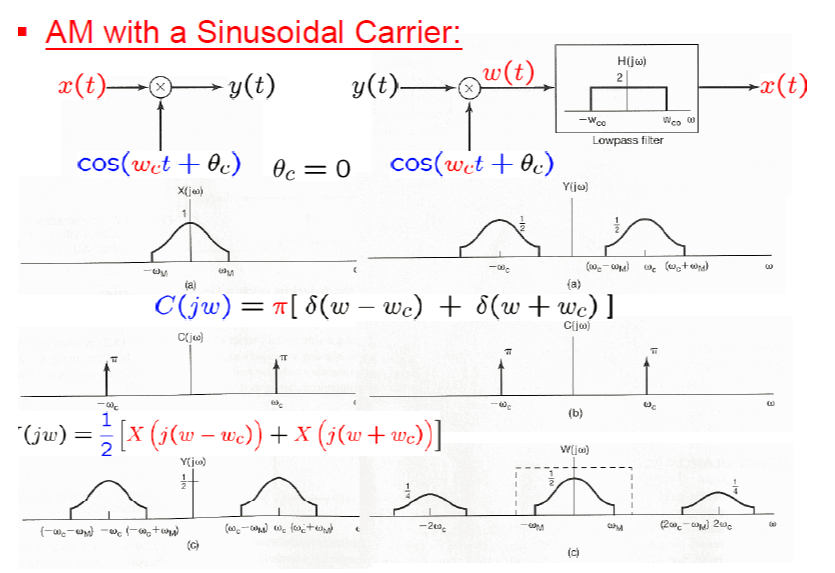
\includegraphics[width=\linewidth]{8.1.2.png}

\subsection{Demodulation for Sinusoidal AM}

\subsubsection{Synchronous Demodulation}
$$y(t)=x(t)\cos\omega_ct$$
$$w(t)=y(t)\cos\omega_ct$$
$$w(t)=x(t)\cos^2\omega_ct=\frac{1}{2}x(t)+\frac{1}{2}x(t)\cos2\omega_ct$$

\subsubsection{Asynchronous Demodulation}
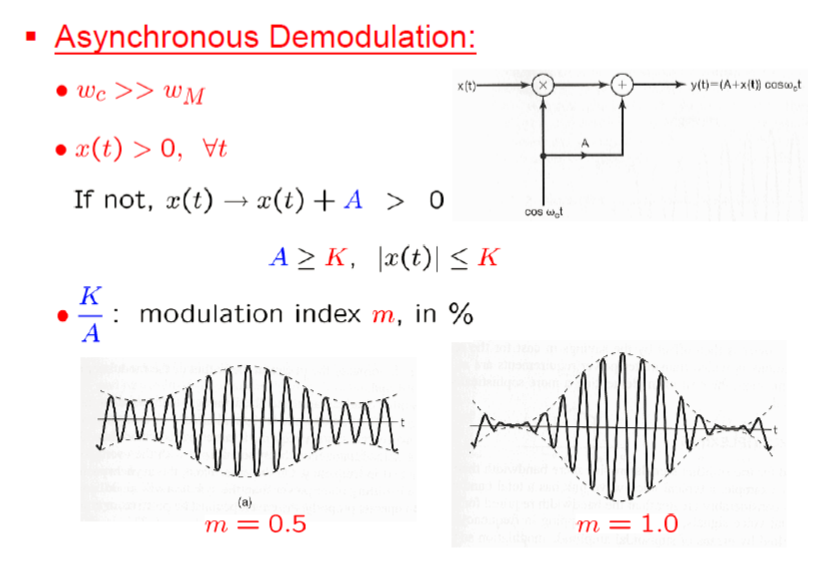
\includegraphics[width=\linewidth]{8.2.2.png}

\subsection{Frequency-Division Multiplexing}
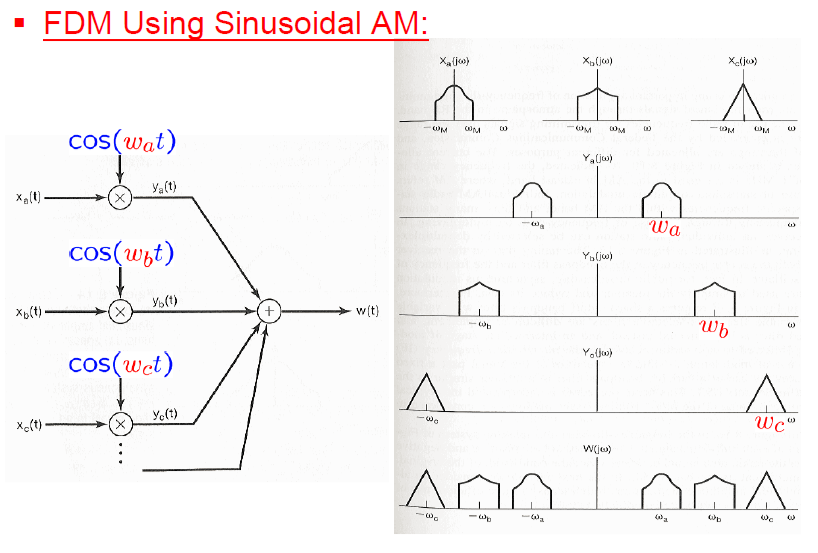
\includegraphics[width=\linewidth]{8.3.png}

\setcounter{section}{10}

\section{Linear Feedback System}
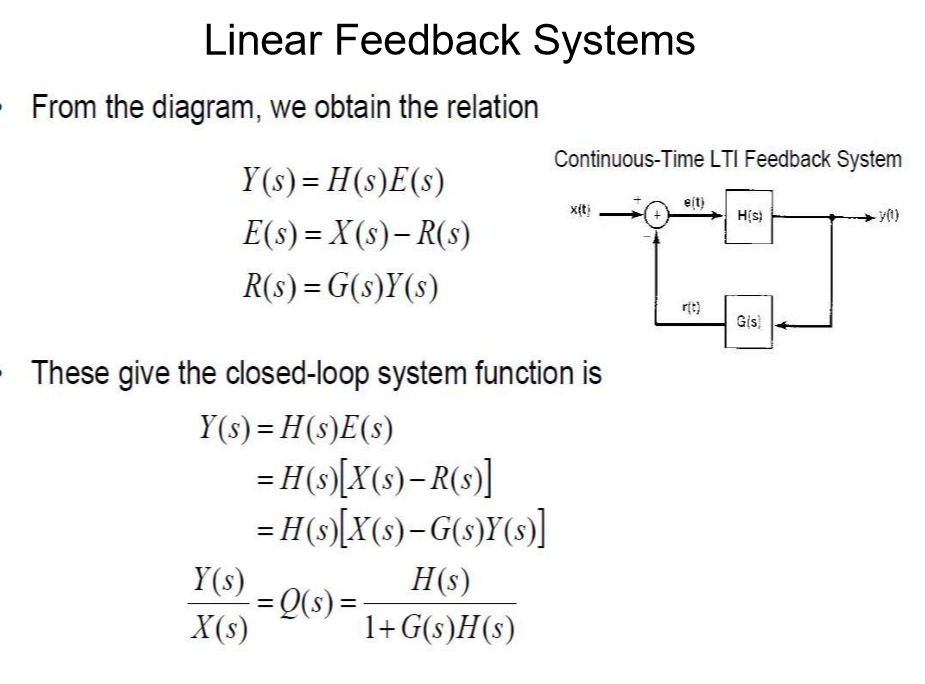
\includegraphics[width=0.8\linewidth]{11.1.png}
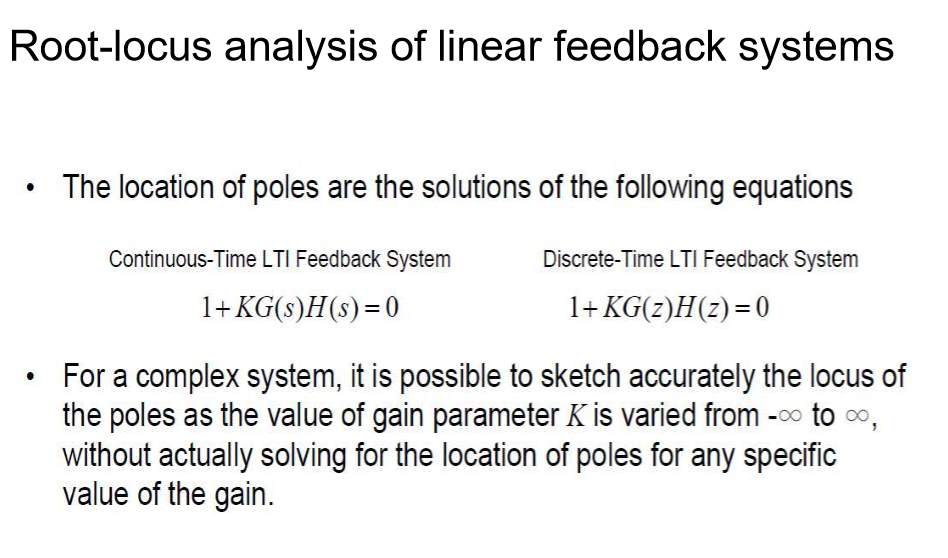
\includegraphics[width=0.8\linewidth]{11.2.png}

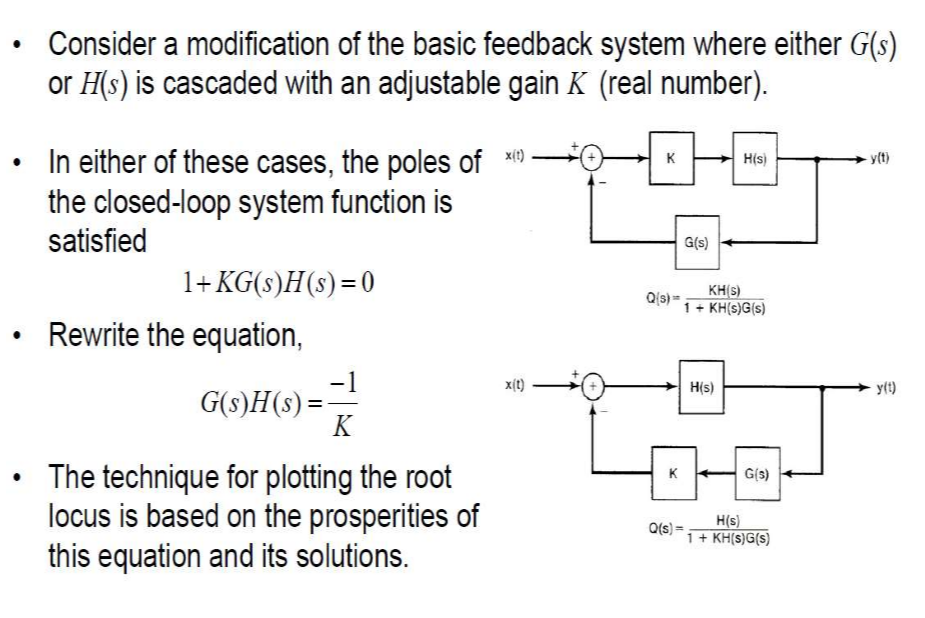
\includegraphics[width=\linewidth]{11.3.png}
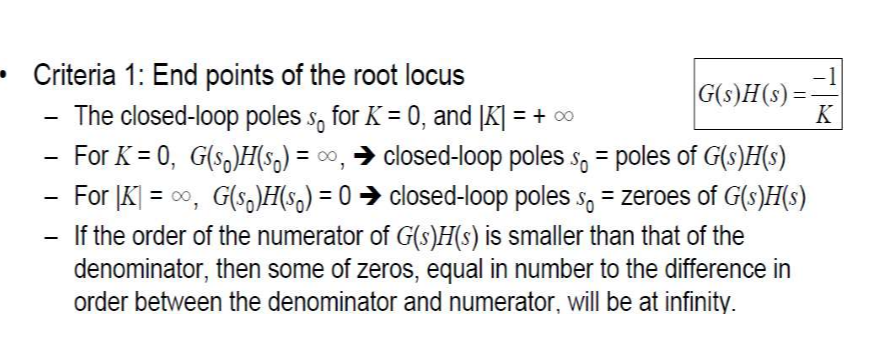
\includegraphics[width=\linewidth]{11.4.png}
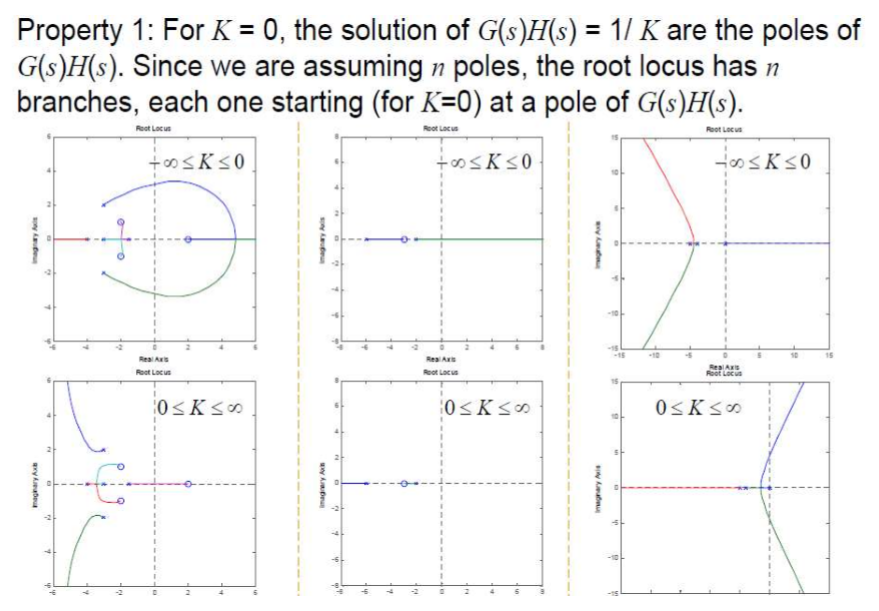
\includegraphics[width=\linewidth]{11.5.png}

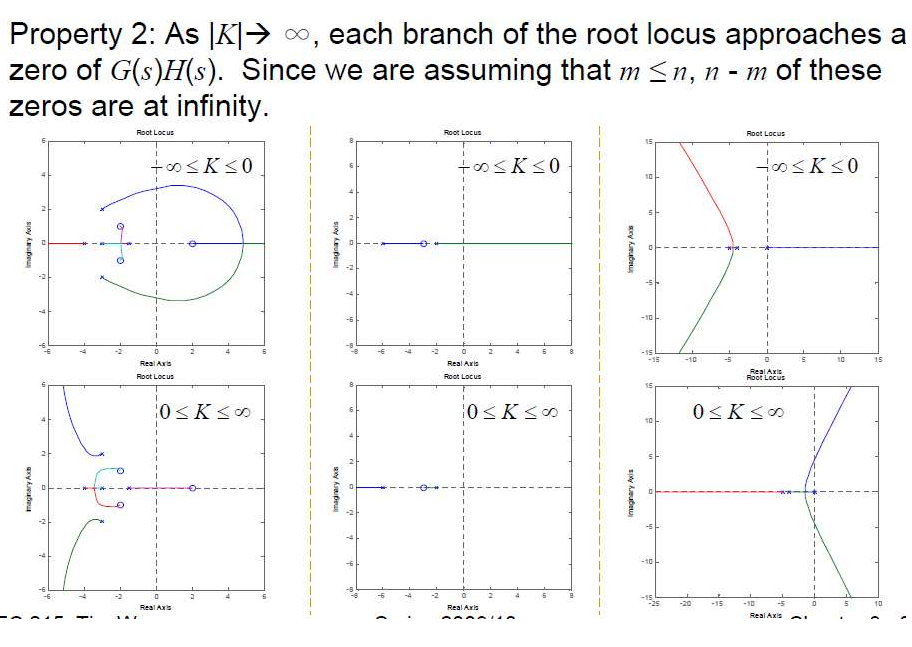
\includegraphics[width=\linewidth]{11.6.png}

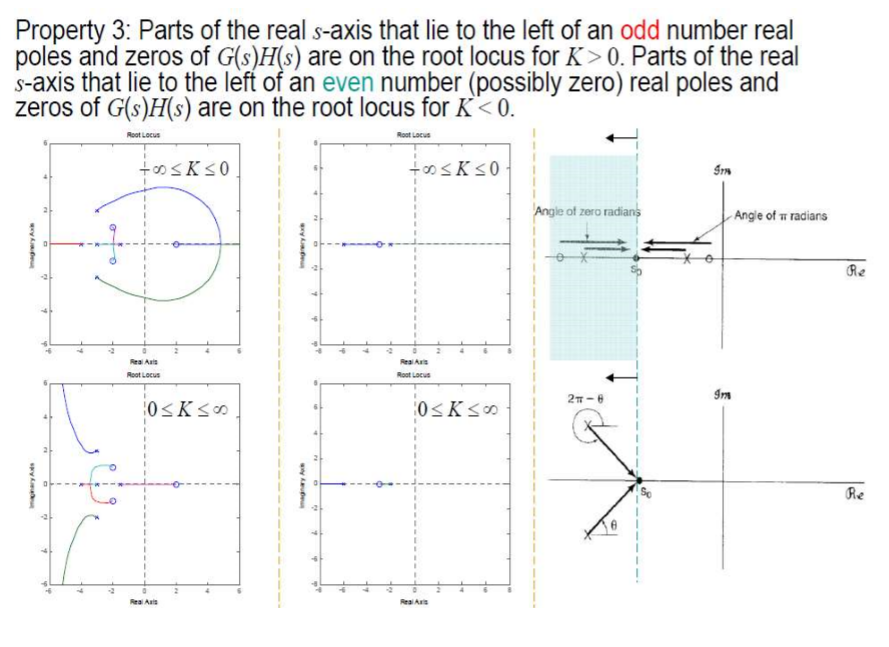
\includegraphics[width=\linewidth]{11.7.png}

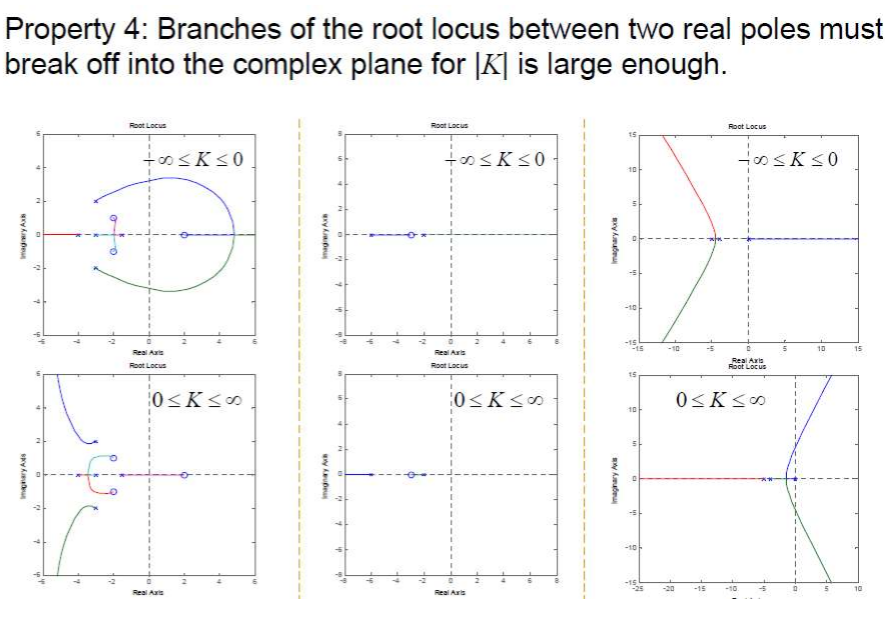
\includegraphics[width=\linewidth]{11.8.png}


\end{multicols}

\setcounter{section}{8}

\newpage
\begin{multicols}{2}
\section{The Laplace Transform}
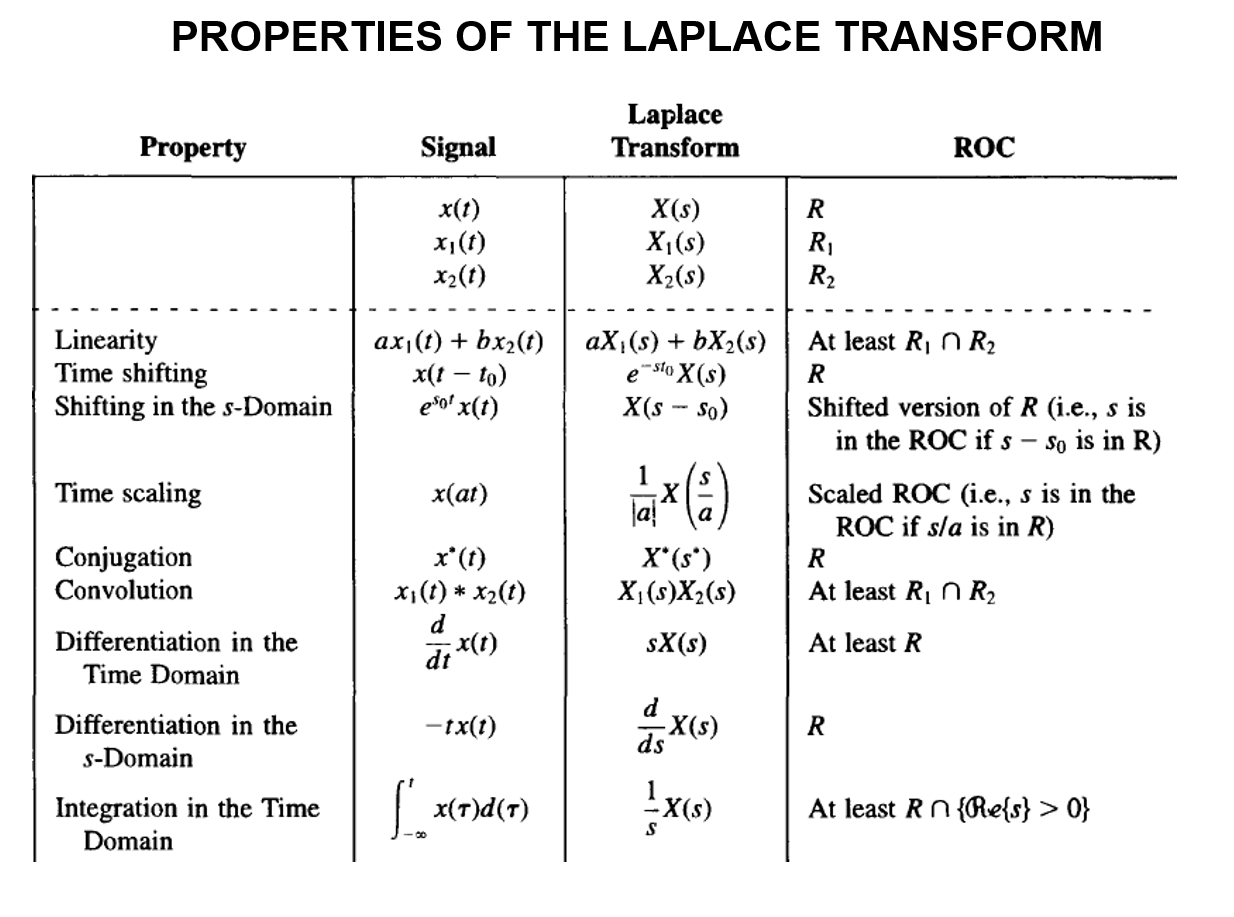
\includegraphics[width=\linewidth]{p1.png}
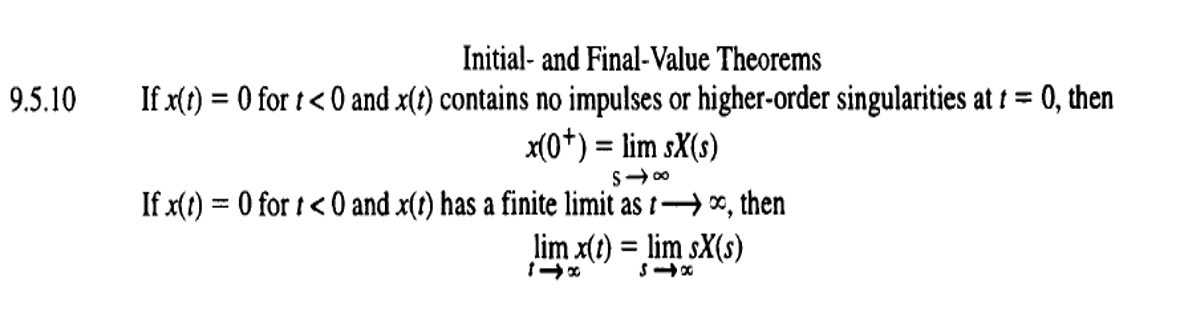
\includegraphics[width=\linewidth]{p7.png}

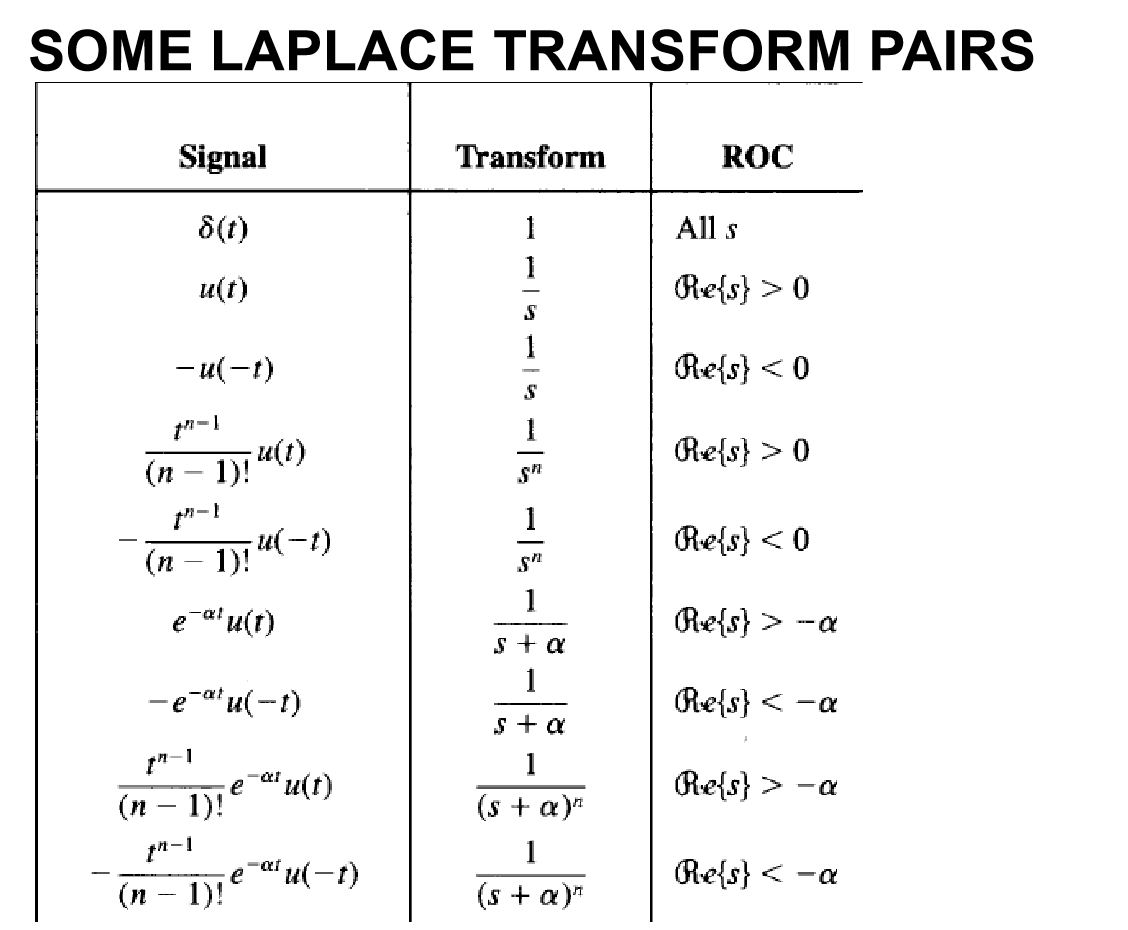
\includegraphics[width=0.9\linewidth]{p2.png}
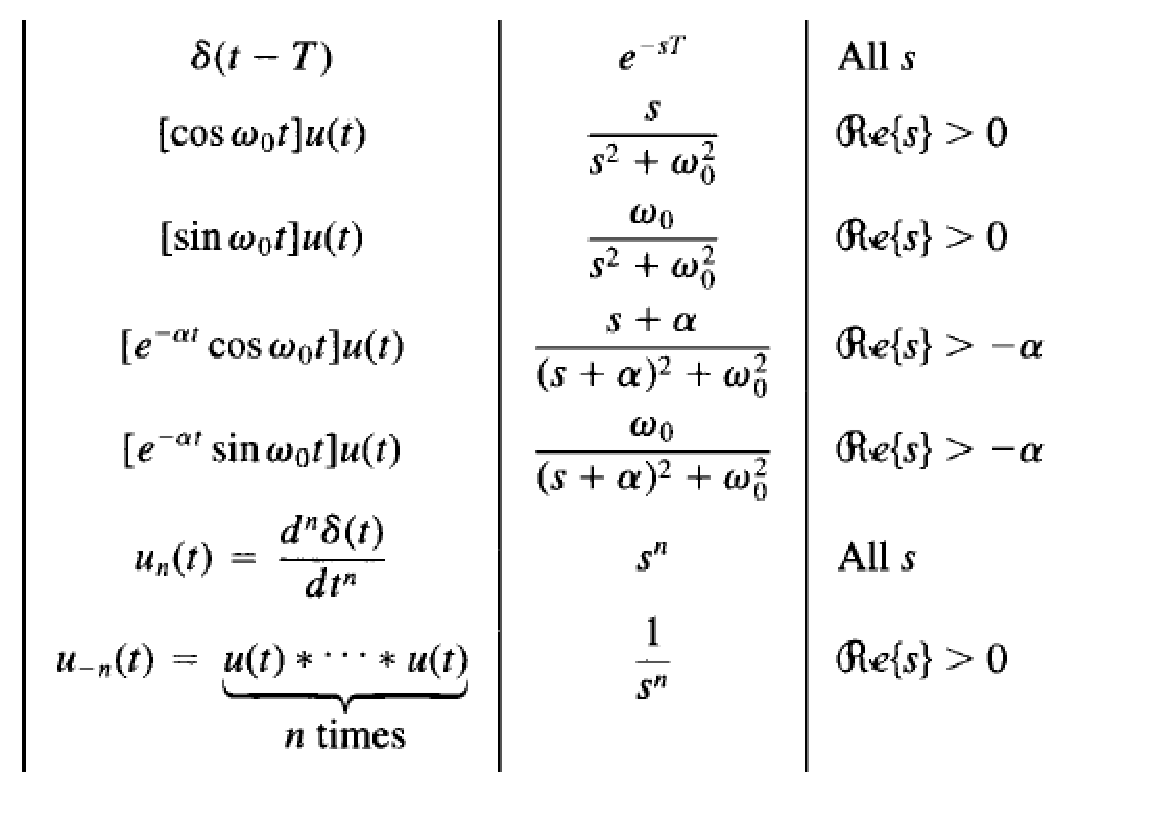
\includegraphics[width=0.9\linewidth]{p3.png}
\end{multicols}

\newpage
\begin{multicols}{2}
\section{The Z-transform}
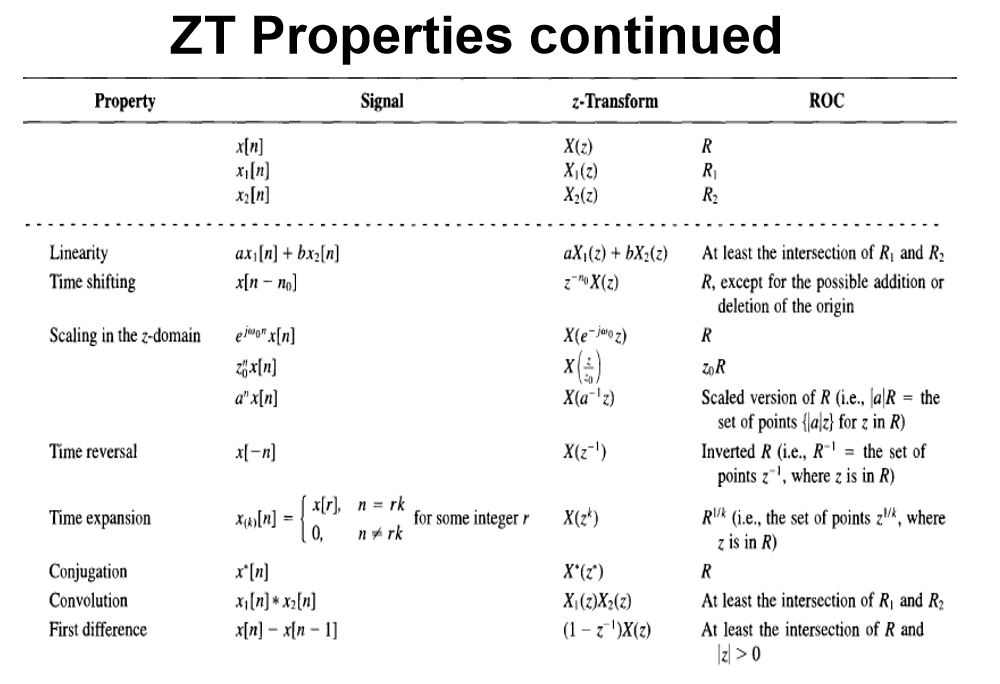
\includegraphics[width=\linewidth]{p4.png}
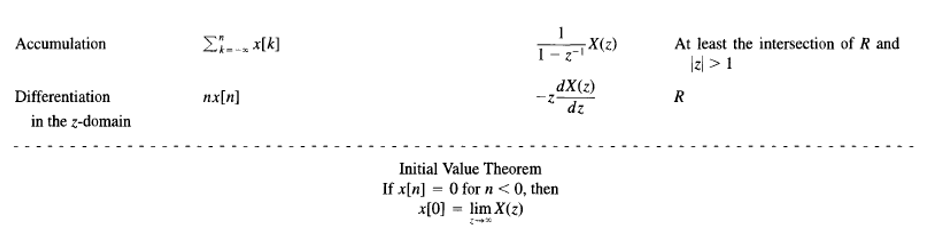
\includegraphics[width=\linewidth]{p5.png}

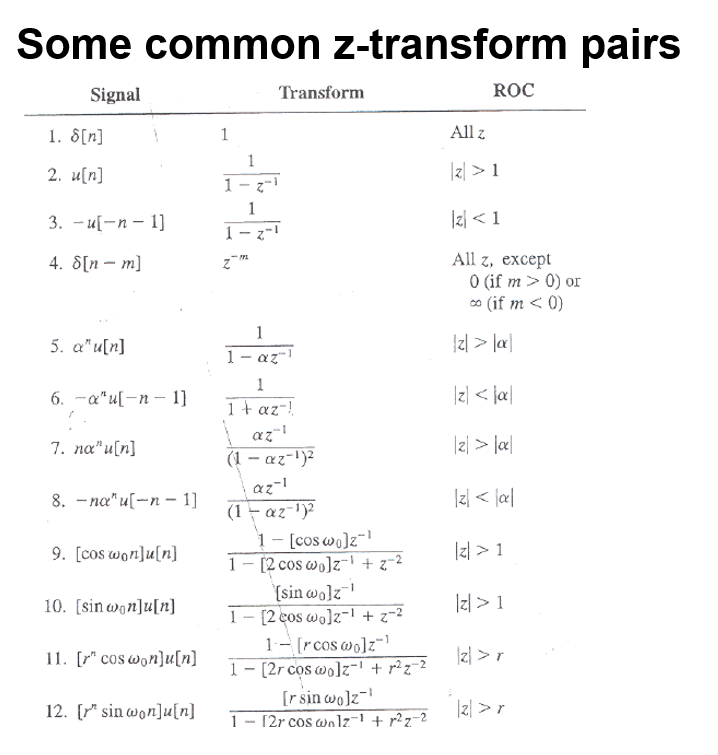
\includegraphics[width=\linewidth]{p6.png}
\end{multicols}

\newpage
\begin{multicols}{2}
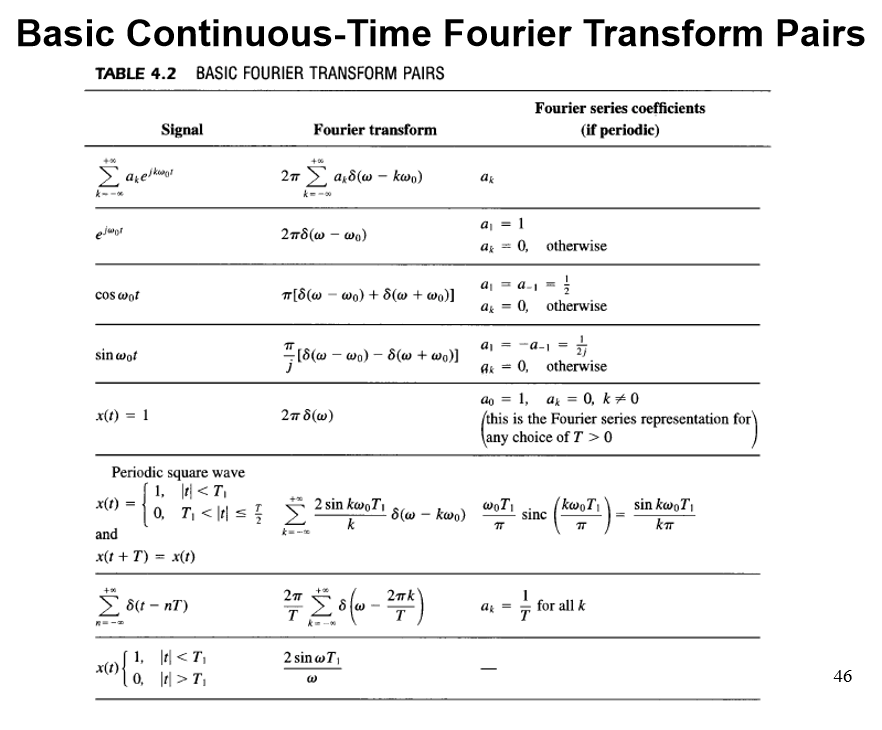
\includegraphics[width=\linewidth]{p8.png}
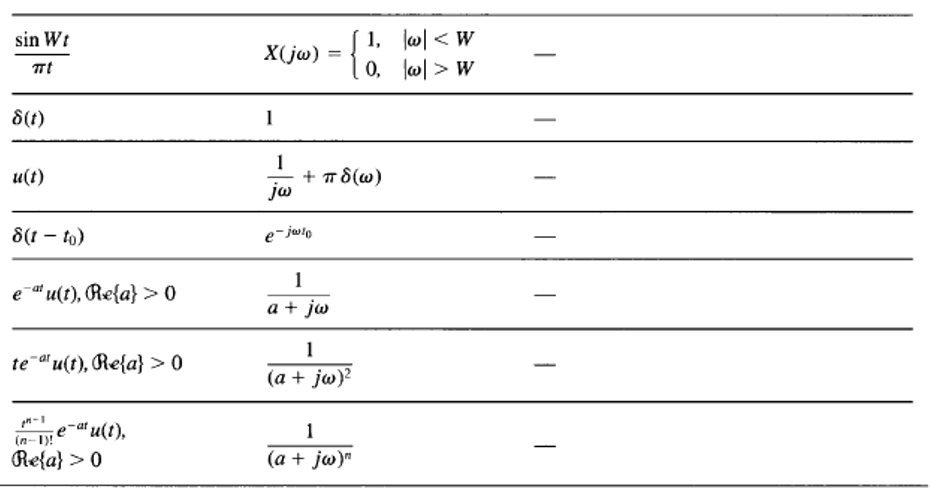
\includegraphics[width=0.9\linewidth]{p9.png}

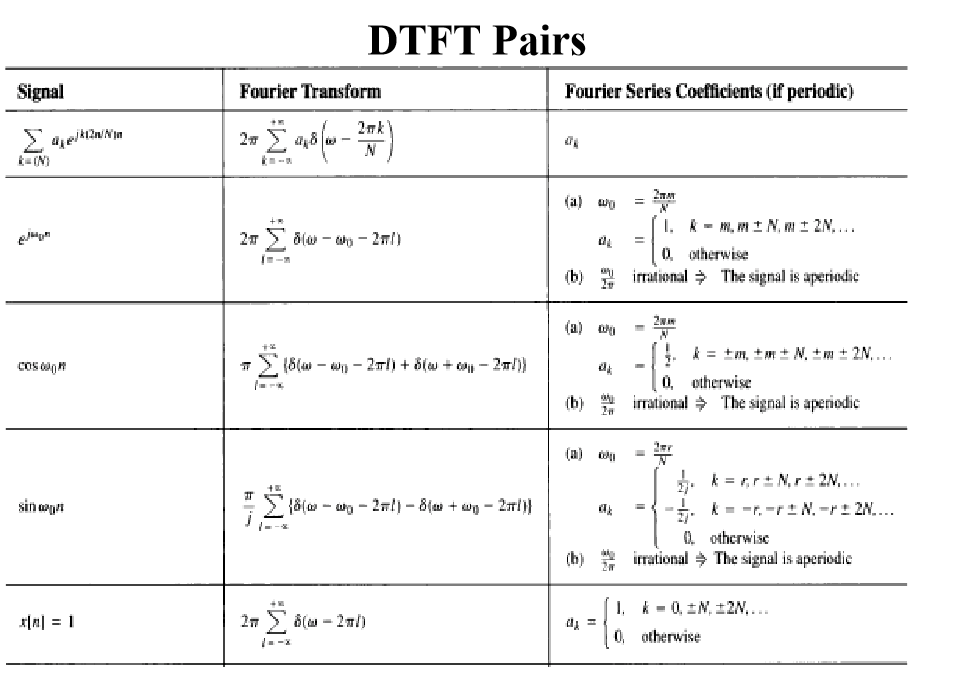
\includegraphics[width=0.9\linewidth]{p10.png}
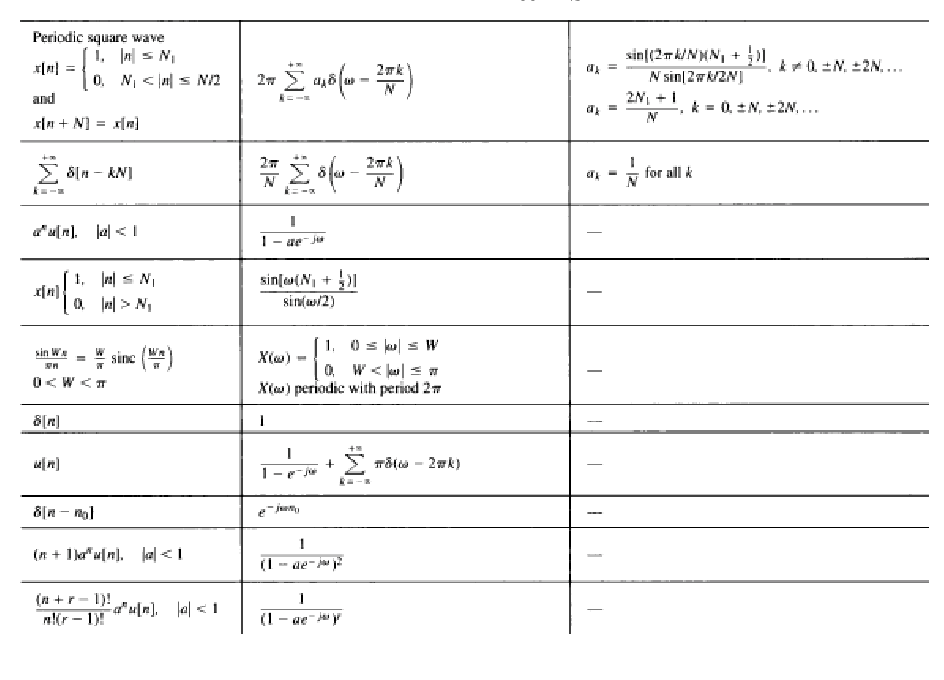
\includegraphics[width=\linewidth]{p11.png}

\end{multicols}

\end{document}
